\documentclass[10pt]{article}
\usepackage{graphicx}
\usepackage[margin=1.5cm]{geometry}
\usepackage{amsmath}
\def\brcurs{{\mbox{$\resizebox{.16in}{.08in}{
\includegraphics{BoldR}}$}}}
\def\rcurs{{\mbox{$\resizebox{.16in}{.08in}{
\includegraphics{ScriptR}}$}}}

\begin{document}
\twocolumn

\title{Thursday Warm-up: Ohm's Law, Electromotive Force (emf), Motional emf}
\author{Prof. Jordan C. Hanson}

\maketitle

\begin{figure}
\centering
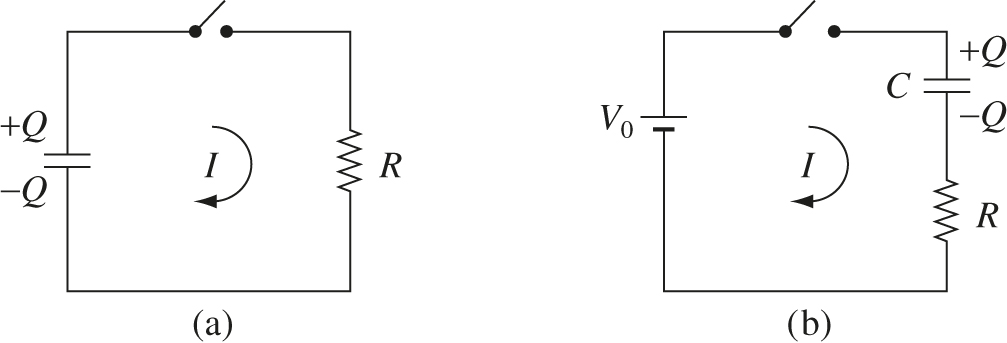
\includegraphics[width=0.49\textwidth]{figures/7_5.jpg}
\caption{\label{fig:1} (Left) A charged capacitor drives current through a resistor. (Right) An emf charges a capacitor, and drives current through a resistor.}
\end{figure}

\section{Memory Bank}

\begin{itemize}
\item \textbf{Ohm's Law}, low-speed charges, small $\mathbf{B}$-fields:
\begin{equation}
\mathbf{J} = \sigma \mathbf{f} = \sigma \mathbf{E} \label{eq:1}
\end{equation}
The vector $\mathbf{f}$ is the force per unit charge, and $\sigma$ is the \textit{conductivity}.  The parameter $1/\sigma = \rho$ is the \textit{resistivity.}
\item \textbf{Energy stored in a capacitor}:
\begin{equation}
U_{\rm C} = \frac{1}{2}CV^2 = \frac{1}{2}\frac{Q^2}{C}
\end{equation}
\item \textbf{Flux rule and emf}:
\begin{align}
\mathcal{E} &= -\frac{d\Phi}{dt} \\
\Phi &= \int \mathbf{B} \cdot d\mathbf{a}
\end{align}
\end{itemize}

\section{Ohm's Law and Motional emf}

\begin{enumerate}
\item Starting with Eq. \ref{eq:1}, show that a conductor with fixed cross-sectional area $A$, potential difference $\Delta V$ between the ends, and current $I$, that
\begin{equation}
\Delta V = I R
\end{equation}
The parameter $R$ should be related to the resistivity. \\ \vspace{1cm}
\item A capacitor $C$ has been charged up to a potential $V_0$ (Fig. \ref{fig:1}, left).  At time $t=0$, it is connected to a resistance $R$. (a) Determine the charge on the capacitor and the current as a function of time. (b) What is the original energy stored in the capacitor? (c) The power from a current $I$ is $P=I^2 R$.  Integrate this to show that energy is conserved. \\ \vspace{3cm}
\item Determine $Q(t)$ and $I(t)$ for the emf in Fig. \ref{fig:1}, right. \\ \vspace{3cm}
\item Suppose the force per unit charge is separated into the force per unit charge from the \textit{source} (battery), and the electrostatic field smoothing the current:
\begin{equation}
\mathbf{f} = \mathbf{f}_s + \mathbf{E}
\end{equation}
The work done on charges all the way around a circuit (emf) is $\oint \mathbf{f} \cdot d\mathbf{l}$.  (a) Show that
\begin{equation}
\mathcal{E} = \oint \mathbf{f} \cdot d\mathbf{l} = \oint \mathbf{f}_s \cdot d\mathbf{l}
\end{equation}
(b) Show that if the \textit{net force} per unit charge $\mathbf{f}$ is zero, that $\Delta V = \mathcal{E}$. \\ \vspace{2.0cm}
\item Suppose the $\mathbf{B}$-field inside a solenoid varies like $B(t) = \mu_0 n I(t)$, where $I(t) = at+b$.  What is the emf induced on a concentric loop of wire with radius $r$ inside the solenoid? 
\end{enumerate}

\end{document}
